\documentclass[10pt,a4paper]{article}

% PDF version and output
\pdfoutput=1        % force the execution of pdflatex
\pdfminorversion=4  % PDF compatibility

% Packages
\usepackage[utf8]{inputenc}
\usepackage{amsmath}
\usepackage{amsfonts}
\usepackage{amssymb}
\usepackage{dsfont}
\usepackage{upgreek}
\usepackage{physics}
\usepackage{graphicx}
% \usepackage{refcheck}

\usepackage{fancyhdr}   % fancy layout

\usepackage{cite}

% Last package to be loaded
\usepackage{bookmark}   % loads hyperref

% Pagestyle (fancyhdr package)
\pagestyle{fancy}
\fancyhead[L]{}
\fancyhead[R]{\small \textsc{\rightmark}}
\fancyfoot[C]{\thepage}
\renewcommand{\headrulewidth}{0.5pt}
\renewcommand{\footrulewidth}{0.5pt}
\fancyheadoffset{0pt}

% Enumerate equations, figures, tables by section
\numberwithin{equation}{section}
\numberwithin{figure}{section}
\numberwithin{table}{section}

% Informations
% Informations
\author{Riccardo Finotello}

\title{
    Machine Learning for Complete Intersection Calabi-Yau 3-folds
    \\[0.3cm]
    \Large{\textbf{Analysis Report: Original Dataset}}
}
\date{\today}

% Hyperref informations
\hypersetup
{
  pdftitle={Machine Learning for Complete Intersection Calabi-Yau 3-folds},
  pdfsubject={Machine Learning},
  pdfauthor={Riccardo Finotello},
  pdfkeywords={machine learning, artificial intelligence, deep learning},
  pdfstartview={FitH},
  pdflang={en-GB},
  pdfpagemode={UseOutlines},
  bookmarksopen={true},
  bookmarksnumbered={true},
  hidelinks
}

\begin{document}
    \maketitle
    
    \begin{abstract}
        In the framework of String Theory, we try to use information available in public datasets concerning configuration matrices of Complete Intersection Calabi-Yau 3-folds to predict the characteristic Hodge numbers $h_{11}$ and $h_{21}$ using machine learning techniques (including neural networks and ensemble learning).
    \end{abstract}
    
    \tableofcontents
    
    \section{Preparation}
        For the first analysis, we considered the original dataset located at \url{http://www.lpthe.jussieu.fr/~erbin/files/data/}: the file was last downloaded on February, 24th 2020 and never directly modified. Before moving to the application of machine learning algorithms and neural networks, we first visualised and analysed the available data in order to extract usable features and gain some insights to be used in the following analysis.

In what follows we use \textit{Scikit-learn} (v.\ 0.22.1), \textit{XGBoost} (v.\ 0.90) and \textit{Keras} (v.\ 2.3.1, with \textit{Tensorflow} v.\ 2.0.0 backend) as reference libraries in a \textit{Conda} installation on \textit{Arch Linux}. Hardware specifications are as follow:
\begin{itemize}
    \item CPU: Intel Core i7-7700HQ @ 2.80 GHz,
    \item GPU: NVIDIA GeForce 940 MX (2 GB RAM),
    \item RAM: 16 GB.
\end{itemize}

\subsection{Data Visualisation}

    After loading the dataset, as a first approach, we considered the distribution in the number of occurrences of $h_{11}$ and $h_{21}$. We considered only manifolds which cannot be represented as products of spaces and we removed some outliers: we considered therefore only entries whose column \texttt{isprod} is identically $0$ and we kept the Hodge numbers in the range $h_{11} \in \left[ 1, 16 \right]$ and $h_{21} \in \left[1, 86 \right]$. We show in Figure~\ref{fig:distribution_occurrences} the distribution of occurrences thus derived. We will then consider the dataset without outliers and product spaces in the following analysis.
    
    \begin{figure}[!t]
        \centering
        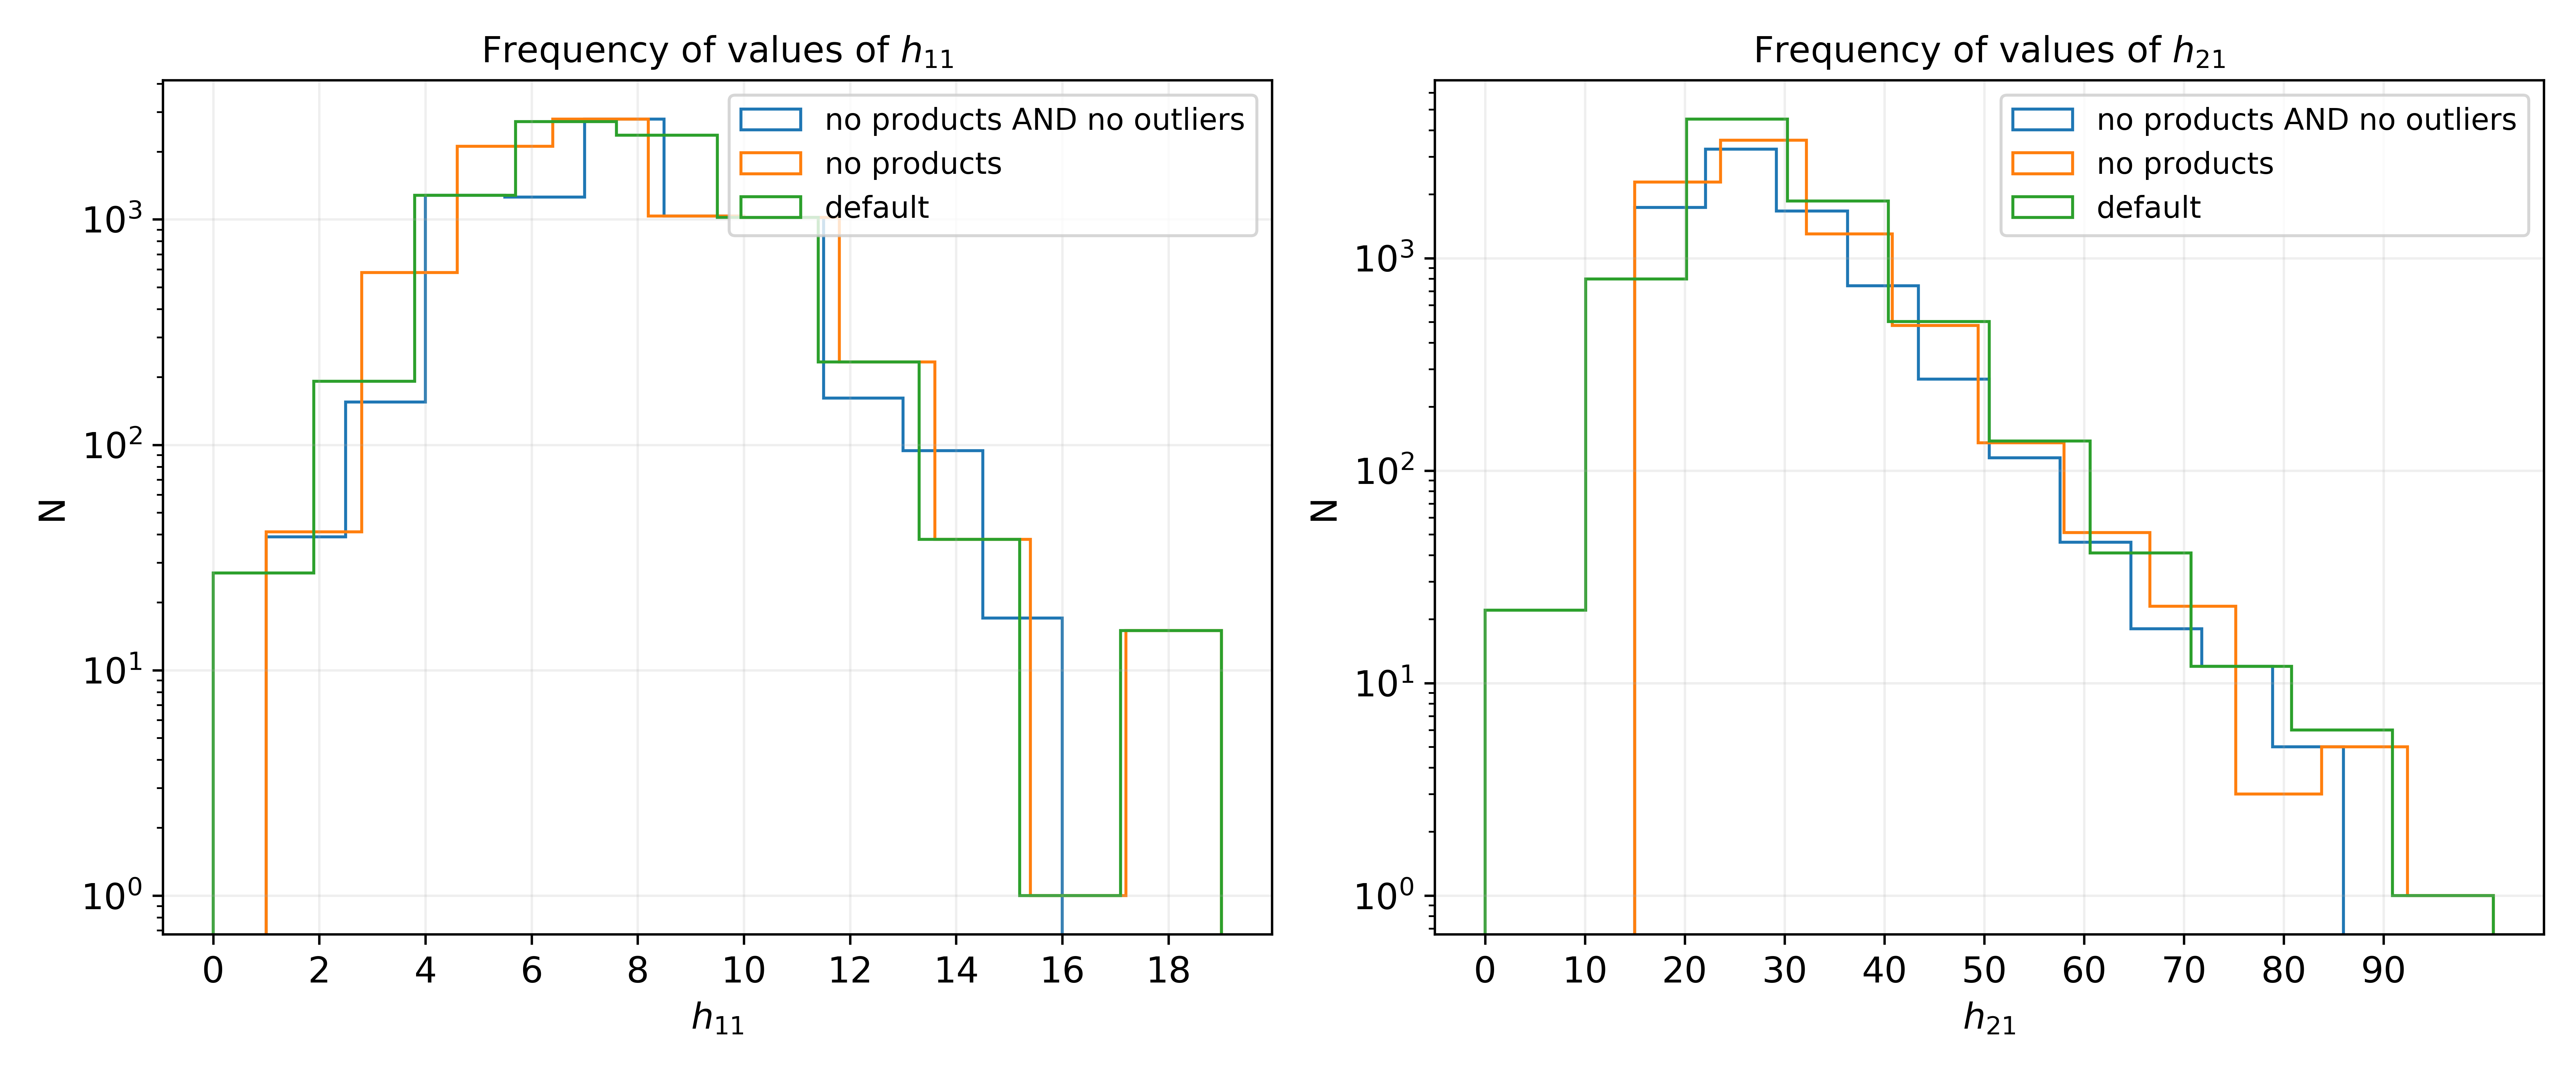
\includegraphics[width=\textwidth]{tex/img/h11_h21_occurrencies.png}
        \caption{Distribution in the number of occurrences of $h_{11}$ and $h_{21}$. The original untouched dataset, the dataset without product spaces and the dataset without outliers are shown in different colours.}
        \label{fig:distribution_occurrences}
    \end{figure}
    
    As a reference, we also plot the distribution of $h_{11}$ and $h_{21}$ with respect to some of the features. Specifically we used \texttt{num\_cp}, \texttt{num\_eqs}, \texttt{norm\_matrix} and \texttt{rank\_matrix} as a reference: relations shown Figure~\ref{fig:scatter_plot_distributions} are not always linear but the distributions of $h_{11}$ and $h_{21}$ show however a tendency to correlation more than sparsity.
    
    \begin{figure}[!t]
        \centering
        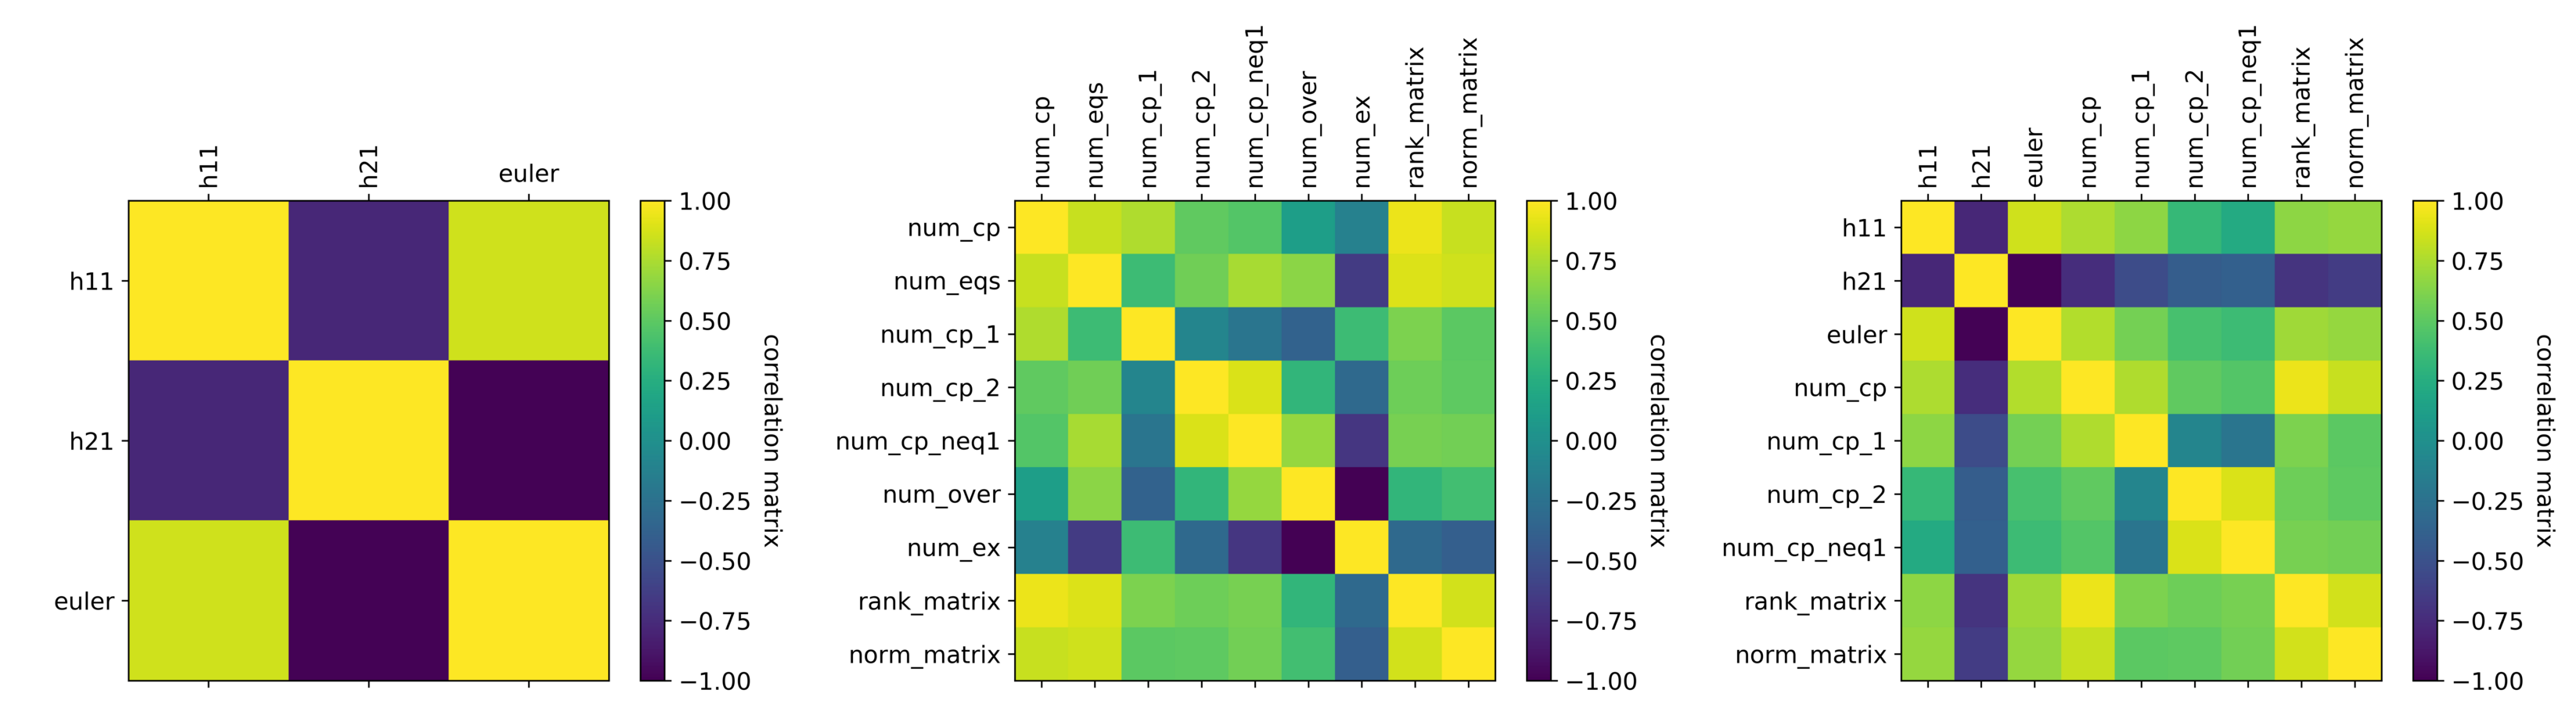
\includegraphics[width=\textwidth]{tex/img/correlation_matrix.png}
        \caption{Correlation matrix of the (scalar) features.}
        \label{fig:correlation_matrix}
    \end{figure}
    
    This can also be inferred from the correlation matrix in Figure~\ref{fig:correlation_matrix} which shows the relations between the labels \texttt{h11}, \texttt{h21} and \texttt{euler} (the latter will not be considered in the analysis) and with respect to other scalar features.
    
    \begin{figure}[p]
        \centering
        \includegraphics[height=0.9\textheight,
                         trim={0 0 6in 0},
                         clip
                        ]{tex/img/h11_h21_distributions.png}
        \caption{Distribution of $h_{11}$ and $h_{21}$ with respect to a restricted number of available features.}
        \label{fig:scatter_plot_distributions}
    \end{figure}
    
\subsection{Clustering and PCA}

    To improve the predictive abilities of the algorithms, we employ a clustering analysis (unsupervised) on the components of the configuration matrix in the hope to find possible associations amongst the entries of the dataset. Since we are not interested in predictions, we use the entire dataset and consider the assigned labels as a new feature for the dataset. In particular we considered K-Means clustering using the \texttt{KMeans} algorithm (\texttt{random\_state} = 42). We ran the algorithm several times in a range of clusters between 2 and 19 and added the labels to the dataset to be later analysed.
    
    \begin{figure}[!t]
        \centering
        \includegraphics[width=\textwidth]{tex/img/h11_h21_pca_distribution.png}
        \caption{Principal Components Analysis with two components on the entire dataset.}
        \label{fig:pca_analysis}
    \end{figure}
    
    We then moved to the Principal Components Analysis (unsupervised) of the components of the configuration matrix using the algorithm \texttt{PCA} (\texttt{random\_state} = 42). We first considered the case of only 2 principal components to be used in plots but not in the real analysis. We show in Figure~\ref{fig:pca_analysis} the distribution of $h_{11}$ and $h_{21}$ with respect to such components. For the analysis we focused on keeping the 99\% of the total variance which, from a $12 \times 15$ (180 entries) matrix, led to a vector of 81 components.
    
\subsection{Feature Importances}

    Using the engineered features (including clustering and PCA), we then train a \texttt{RandomForestRegressor}, using the \textit{Scikit-learn} implementation, on the entire dataset (we are still not interested in making predictions) to measure the variable ranking for the different features. The algorithms does not need to be fine tuned at this level of the analysis. We therefore considered the following hyperparameter space\footnote{Here as in the following, hyperparameter which are not explicitely specified are to be considered at their defaults.}:
    \begin{itemize}
        \item \texttt{criterion}: \textit{mse},
        \item \texttt{n\_estimators}: 48,
        \item \texttt{random\_state}: 42.
    \end{itemize}
    Even though it is not relevant for the analysis for many reasons (one above all, it was not computed on a separate training set from which to validate the results before making prediction), the accuracy for $h_{11}$ resulted to be $90.74\%$ and $59.00\%$ for $h_{21}$.
    
    \begin{figure}[!t]
        \centering
        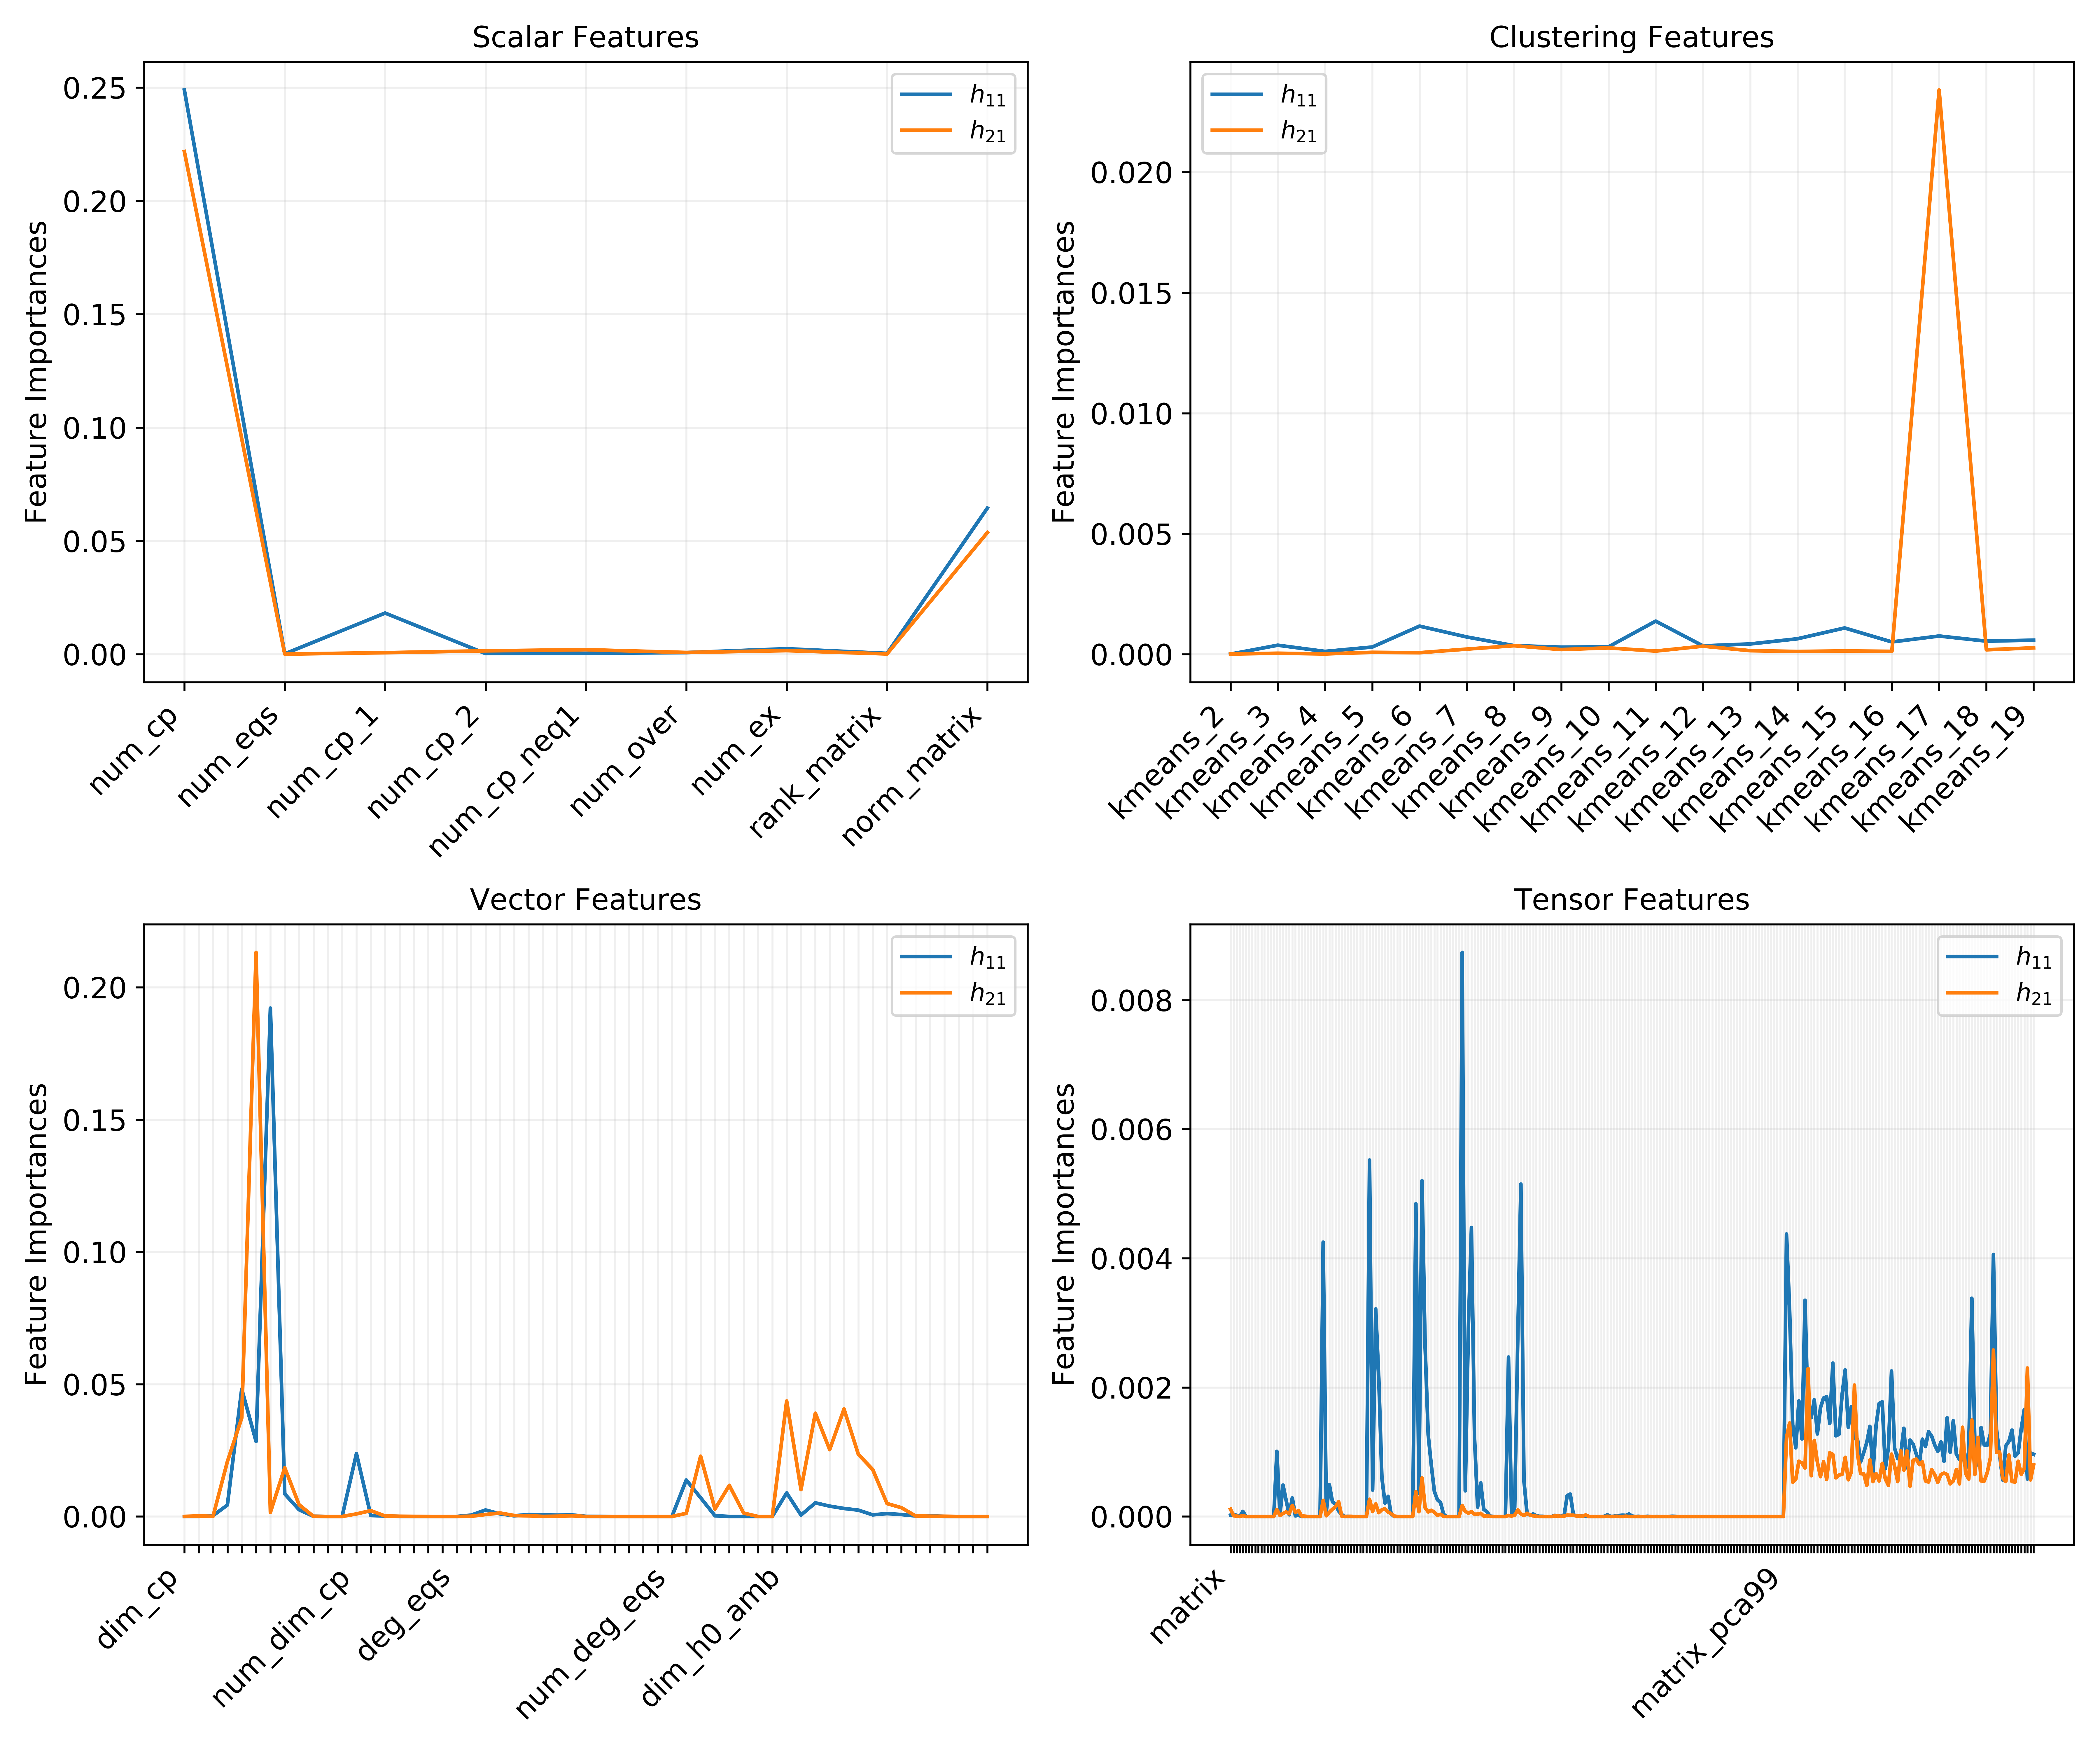
\includegraphics[width=0.75\textwidth,
                         trim={6in 5in 0 0},
                         clip
                        ]{tex/img/feature_importances.png}
        \caption{Clustering ranking.}
        \label{fig:clustering_importances}
    \end{figure}
    
    In Figure~\ref{fig:clustering_importances} we show the ranking of the clustering algorithm which shows that \texttt{KMeans} does not play a role in the prediction of $h_{11}$ while it is only marginally relevant for $h_{21}$. The number of clusters needed is however unrelated to any other feature and varies a lot in relation to the random seed initially set (42 in the case reported here).
    
    \begin{figure}[!t]
        \centering
        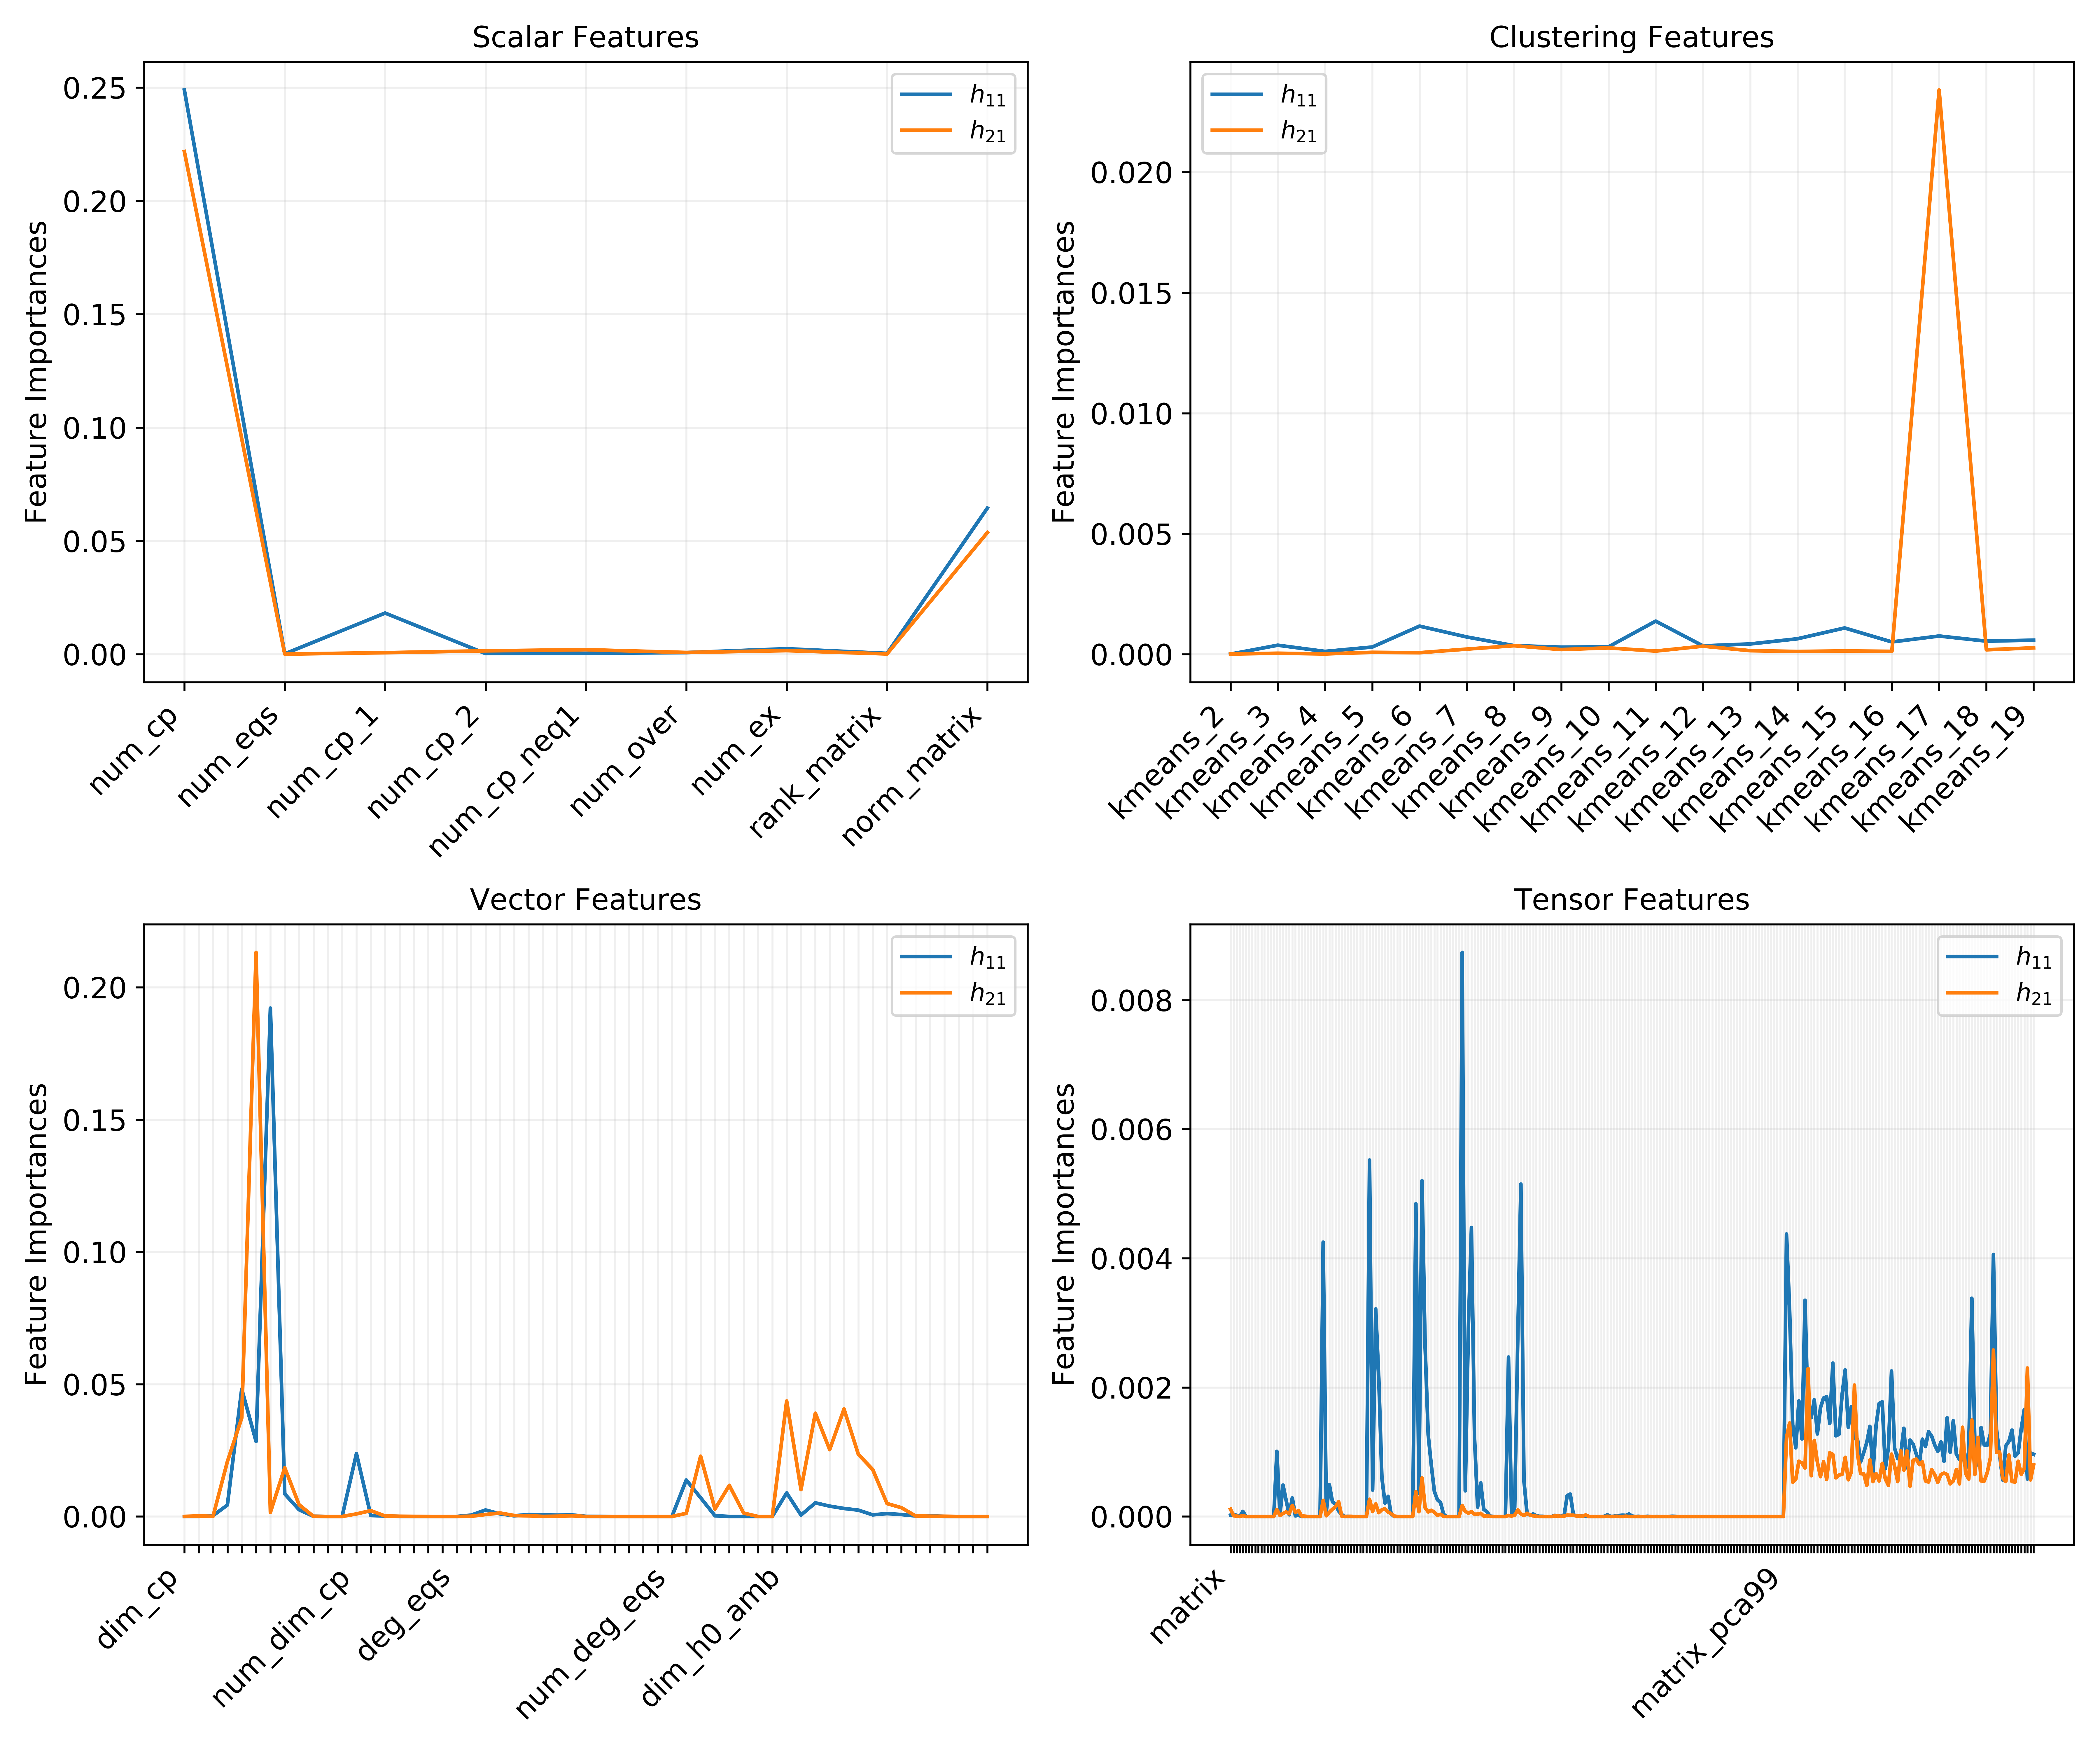
\includegraphics[width=0.75\textwidth,
                         trim={0 5in 6in 0},
                         clip
                        ]{tex/img/feature_importances.png}
        \caption{Scalar ranking.}
        \label{fig:scalar_importances}
    \end{figure}
    
    \begin{figure}[!t]
        \centering
        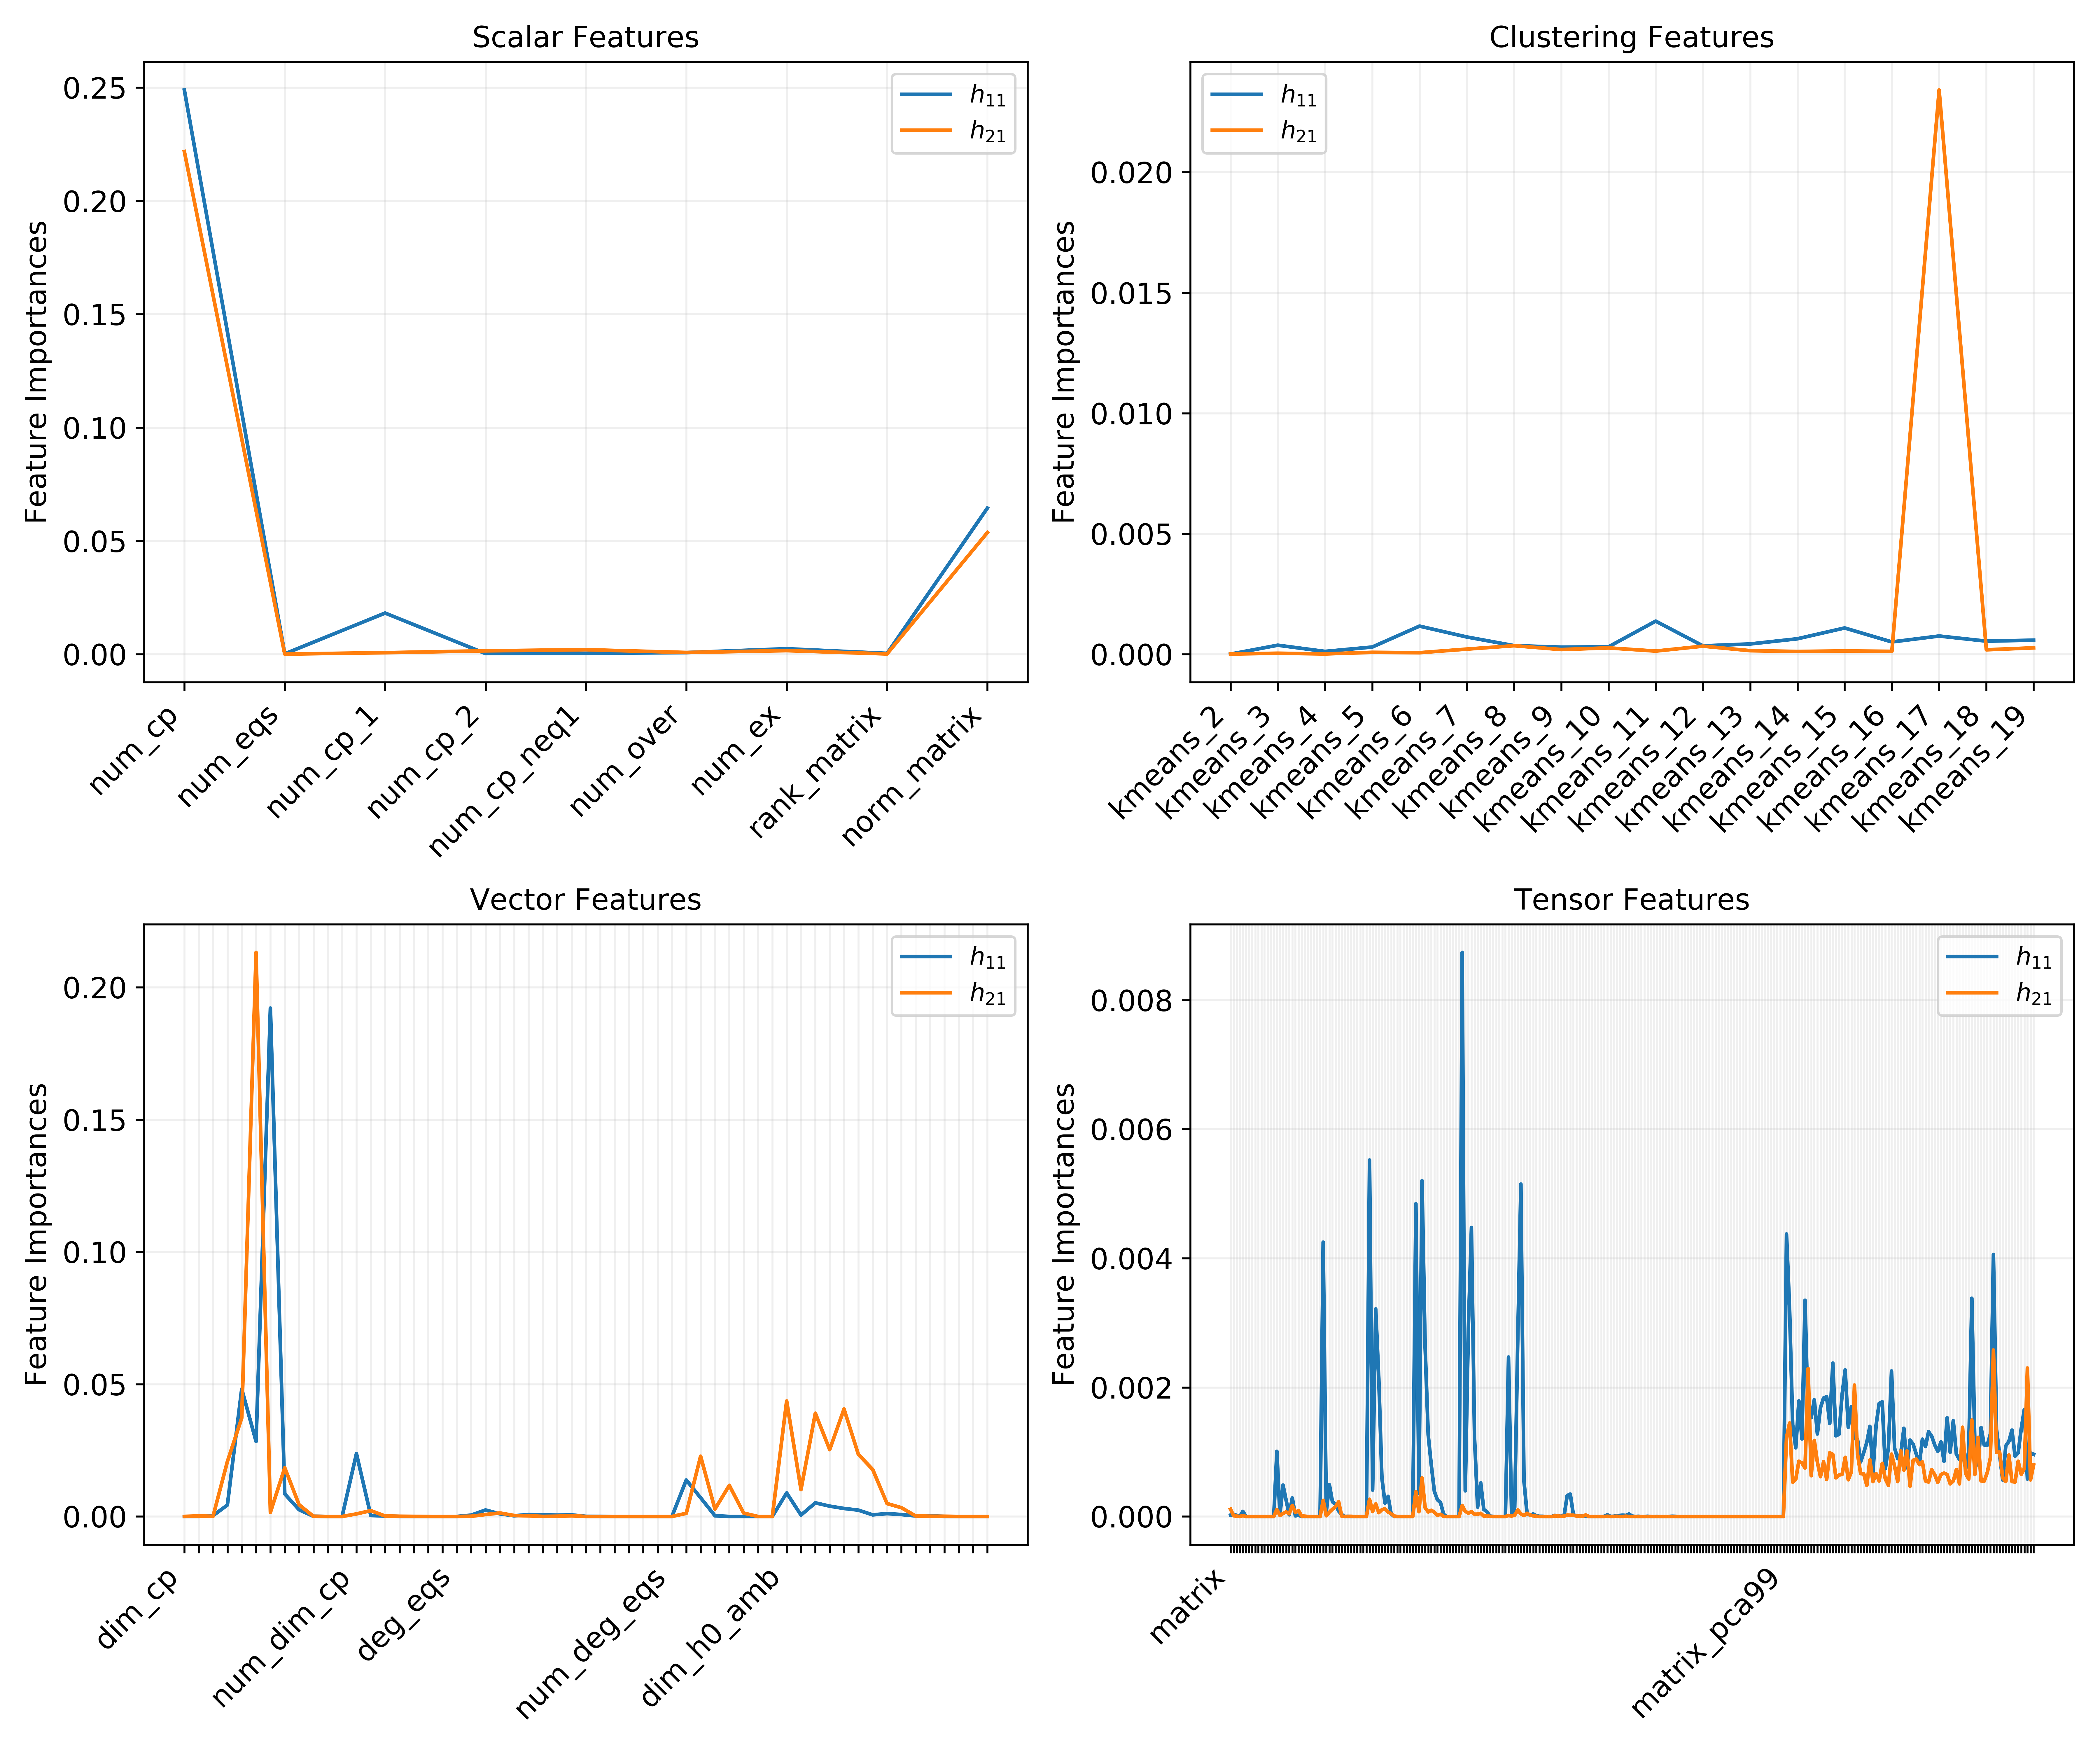
\includegraphics[width=\textwidth,
                         trim={0 0 0 5in},
                         clip
                        ]{tex/img/feature_importances.png}
        \caption{Vector and tensor ranking.}
        \label{fig:vector_tensor_importances}
    \end{figure}
    
    \begin{figure}[!t]
        \centering
        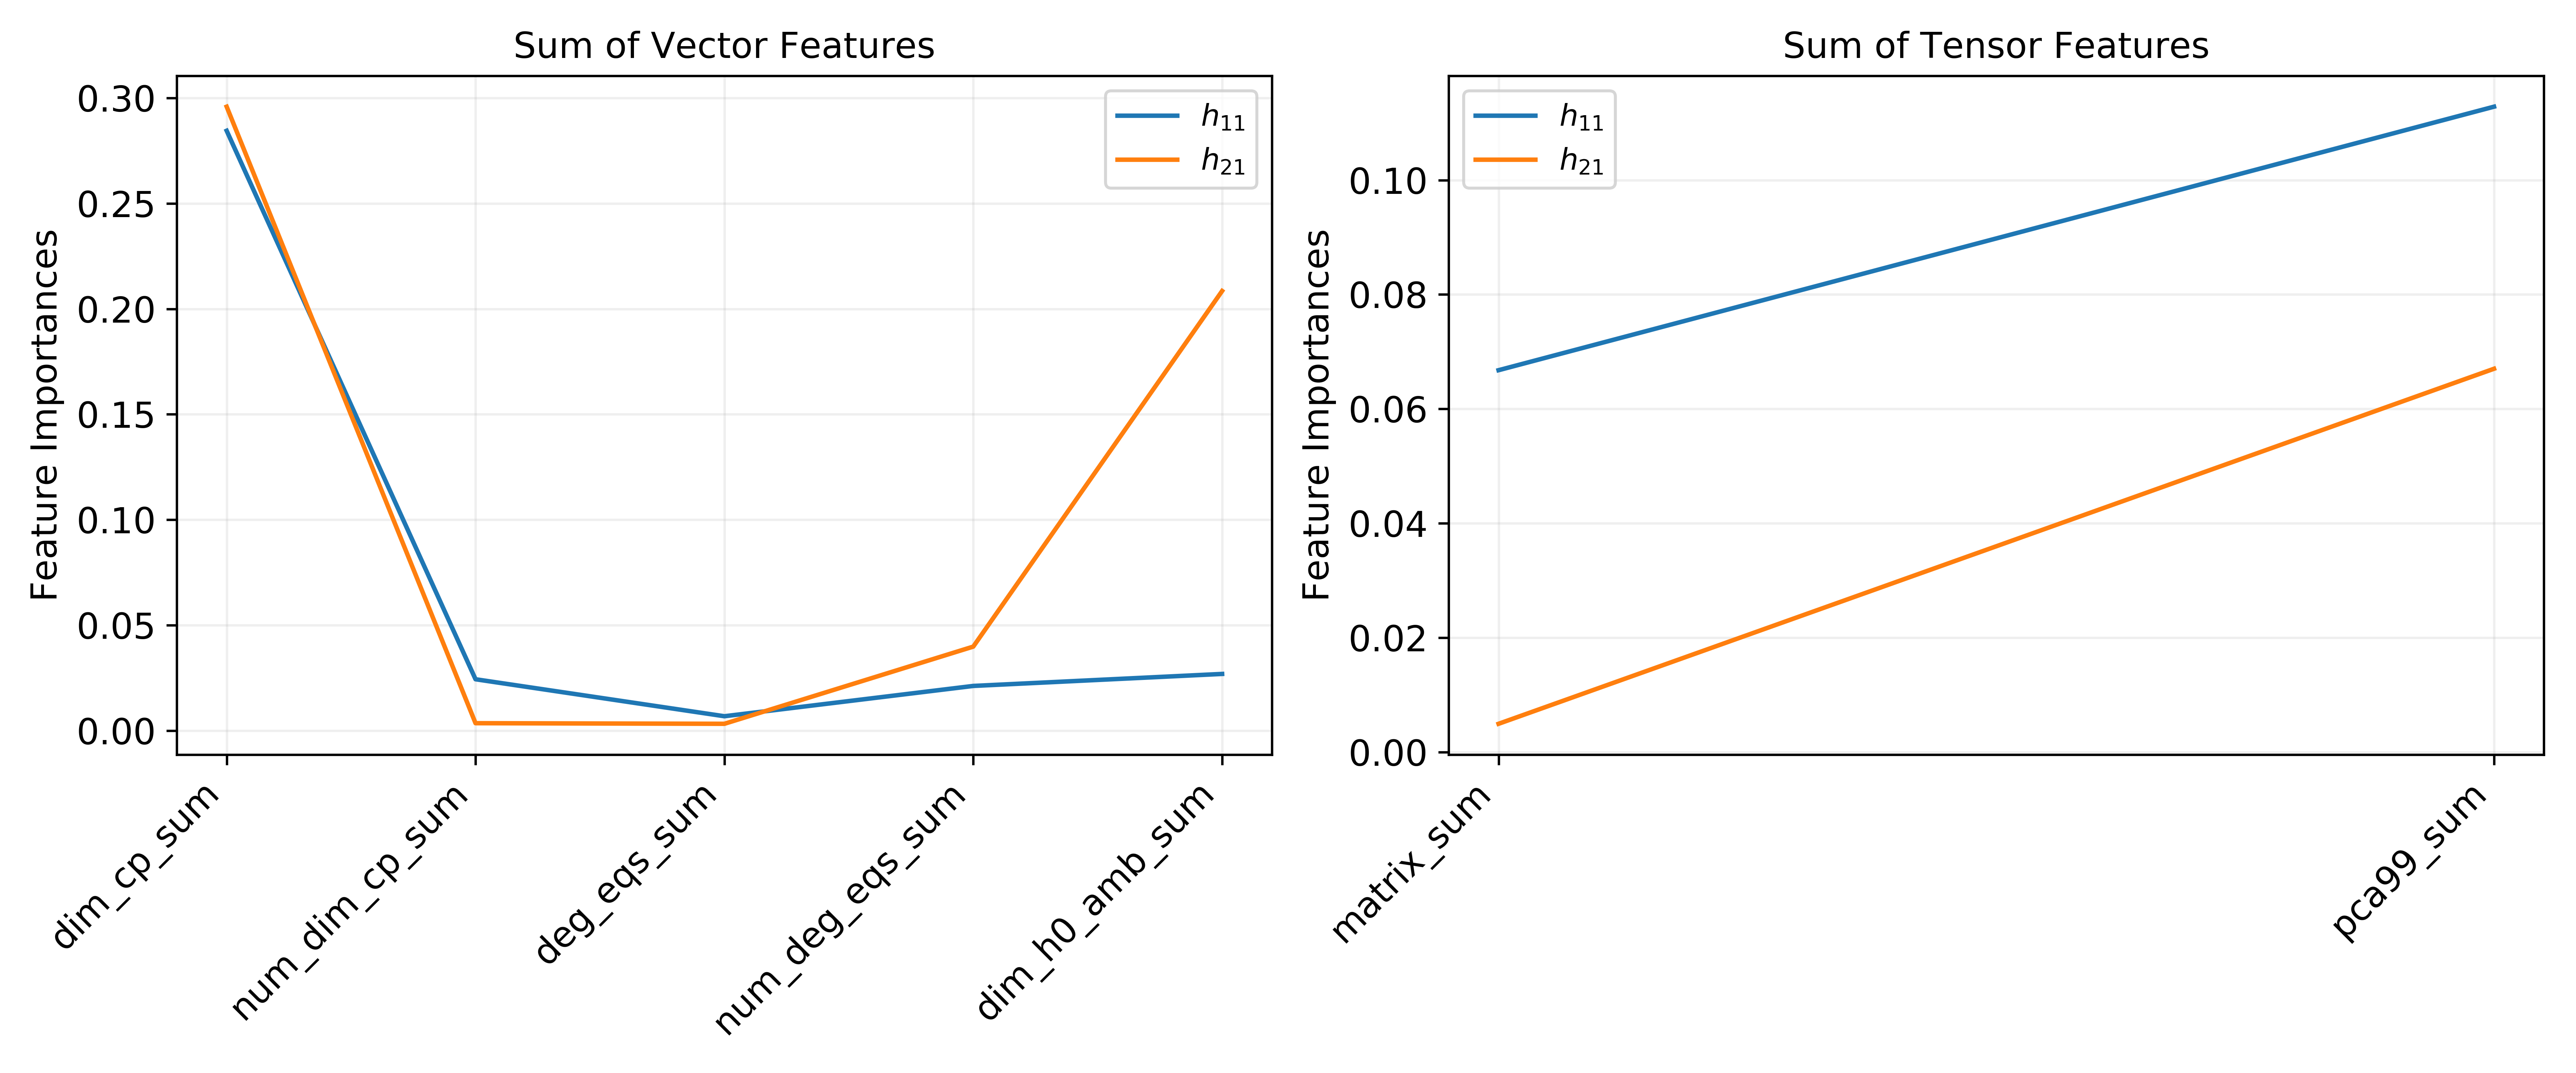
\includegraphics[width=\textwidth]{tex/img/feature_importances_vector_tensor_sum.png}
        \caption{Sum of vector and tensor ranking.}
        \label{fig:vector_tensor_sum_importances}
    \end{figure}
    
    In Figure~\ref{fig:scalar_importances} we show the importance related to the other scalar features, thus showing that only a few of them will actually play a relevant role in the determination of the labels. The same also applies to the vector and tensor features (shown in Figure\ref{fig:vector_tensor_importances} by components): while it may be simpler to show the sum of the importance of the components (as in Figure~\ref{fig:vector_tensor_sum_importances}), it is already clear that the \texttt{PCA} is more relevant than the plain matrix. We then show in Figure~\ref{fig:summary_importances} a summary of the variable ranking.
    
    \begin{figure}[!t]
        \centering
        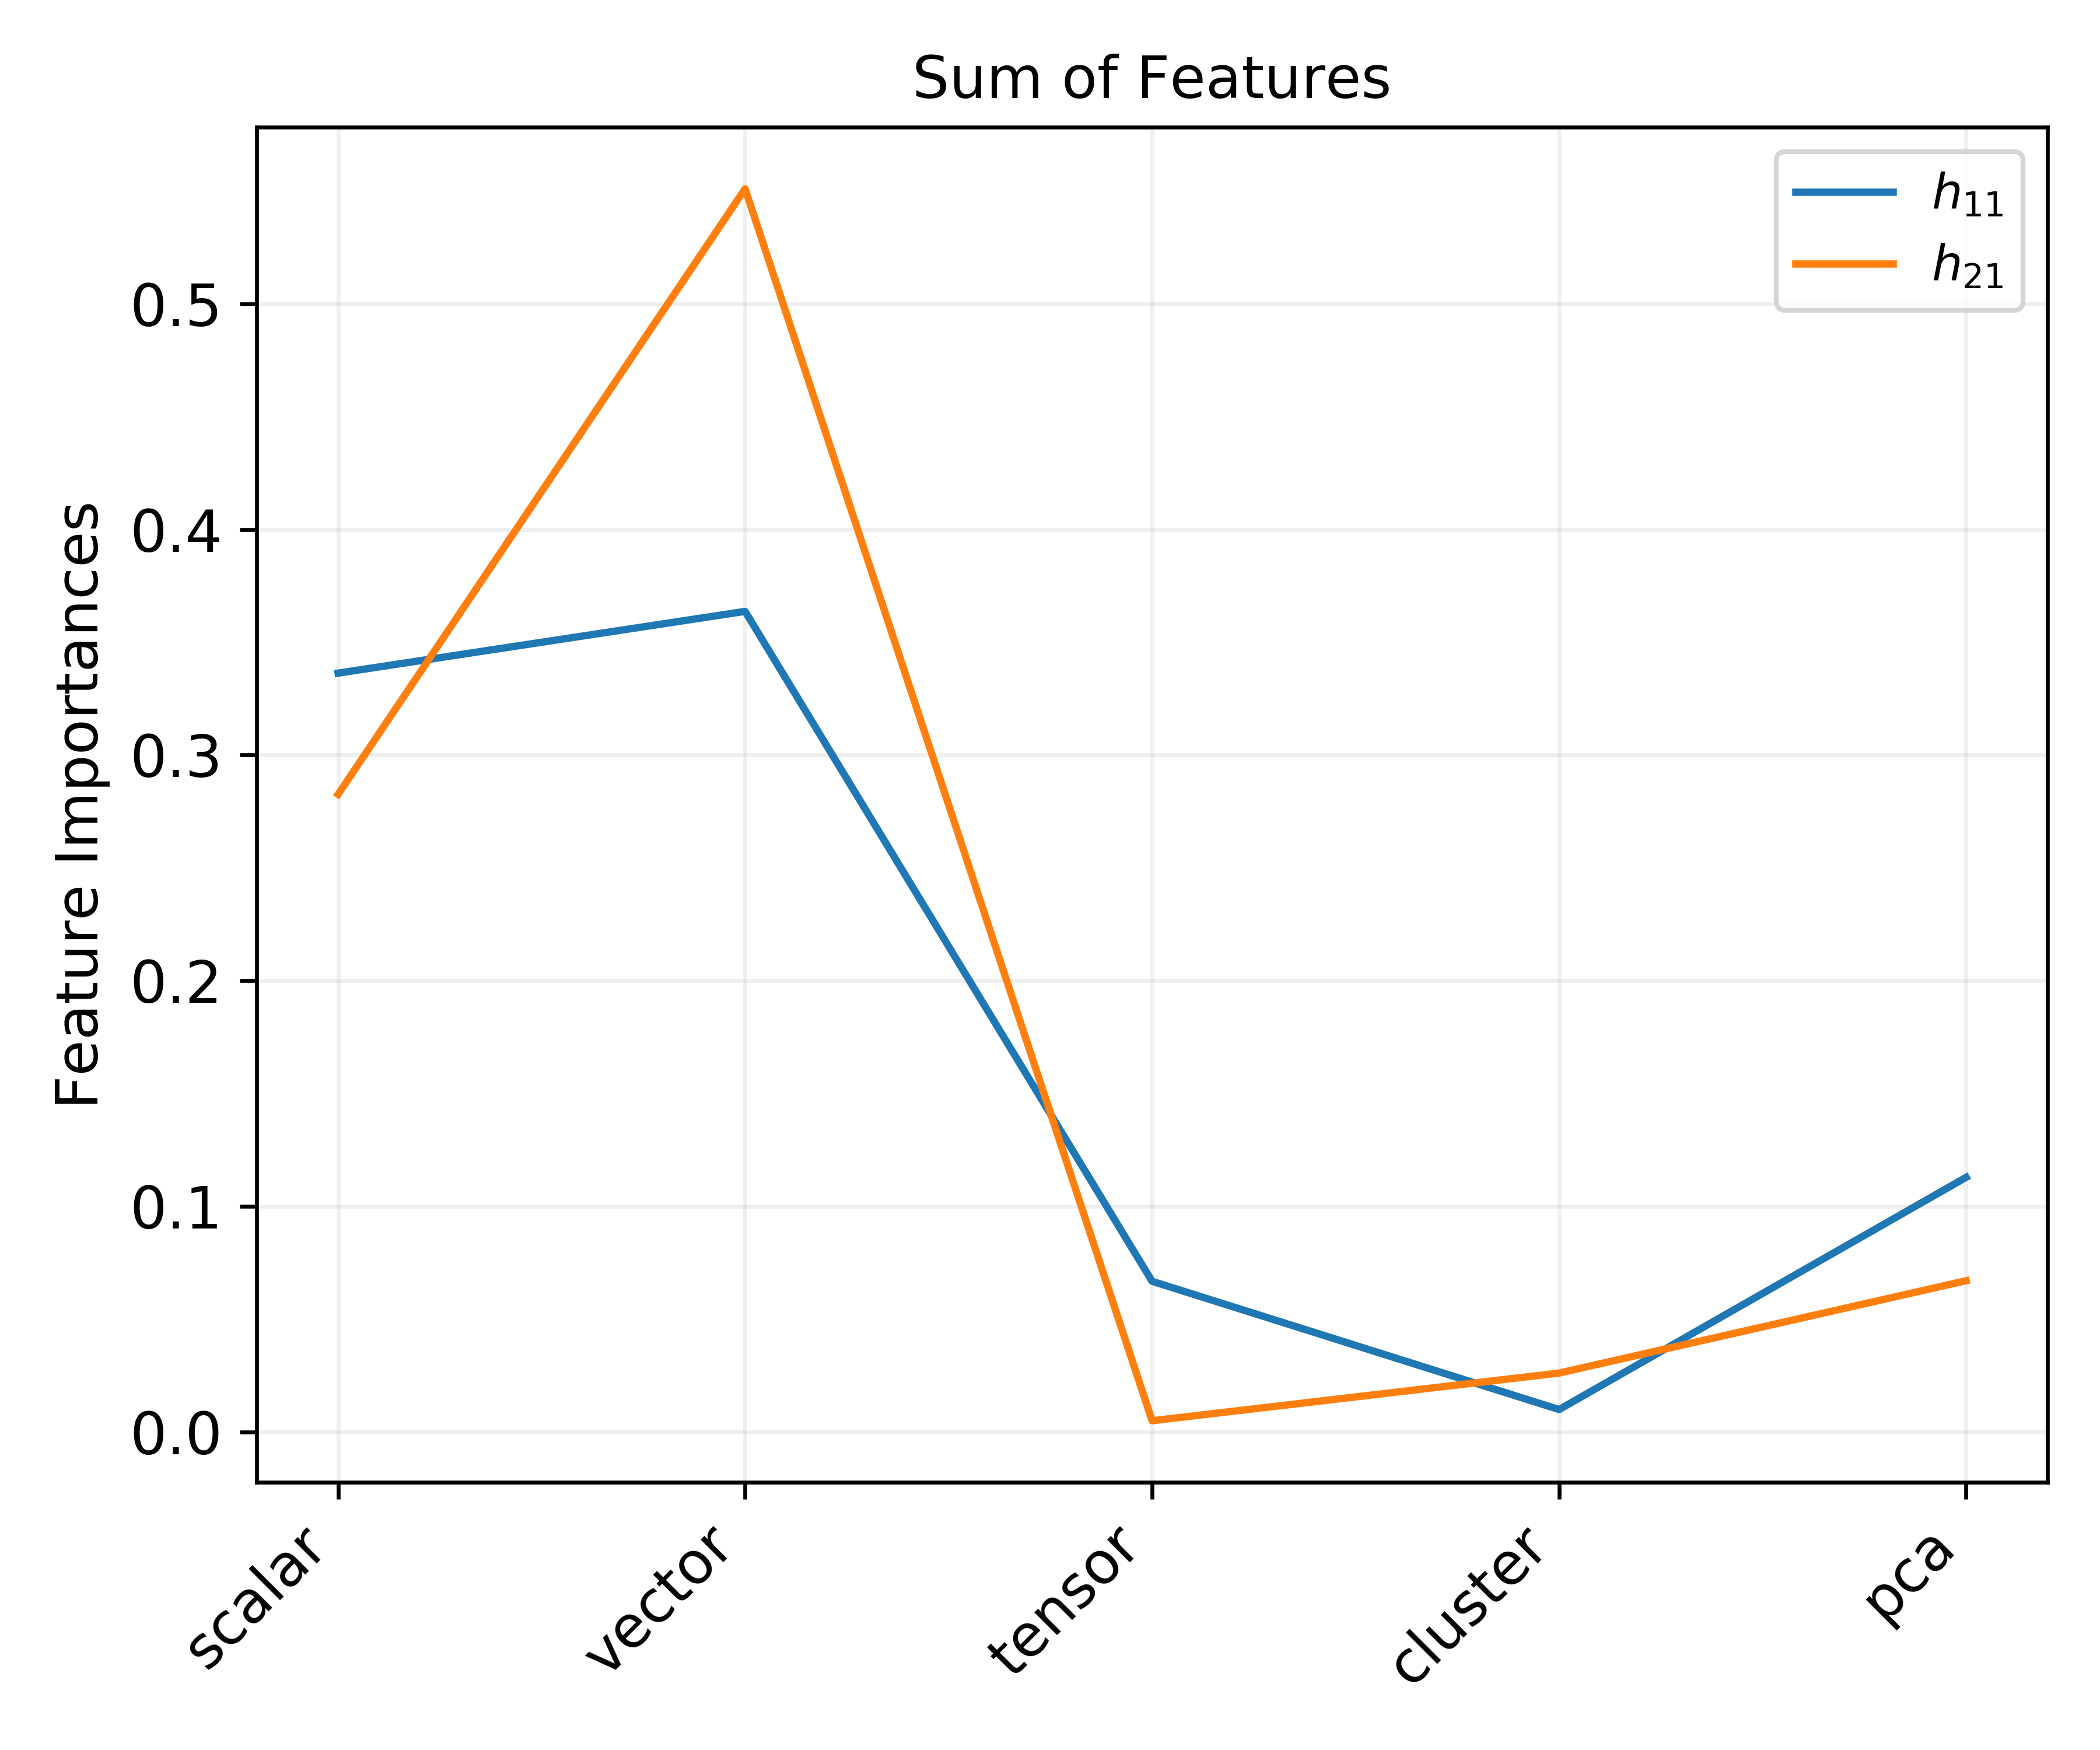
\includegraphics[width=0.75\textwidth]{tex/img/feature_importances_sum.png}
        \caption{Summary of the variable ranking}
        \label{fig:summary_importances}
    \end{figure}
    
\subsection{Feature Selection}

    Using previous results, we then select only the relevant features for the following analysis. In particular we select \texttt{num\_cp}, \texttt{dim\_cp} and the \texttt{PCA} of the configuration matrix for the predictions of $h_{11}$ and \texttt{num\_cp}, \texttt{dim\_cp}, \texttt{dim\_h0\_amb} and the \texttt{PCA} of the configuration matrix for the predictions of $h_{21}$. However we also keep a separate copy of the configuration matrix, \texttt{num\_cp} only and \texttt{dim\_cp} only for comparison during the analysis.
    
    \section{Methodology and Analysis}
        \subsection{Training and Test Sets and Validation Strategy}
    In the analysis we first split the entire dataset into a training and a test subsets. We retain 10\% of the data as test while we take 90\% of the dataset as training set. We also implement cross-validation for the evaluation of the algorithms (not the neural networks): we use a \texttt{KFold} approach with 9 splits, which amount to using 80\% of the total dataset as training set while retaining another 10\% as validation set for each of the 9 folds. For the neural networks we will simply use holdout validation with 10\% of the total data as validation set and 80\% as training.
    
\subsection{Metrics and Evaluation}
    While we are interested in a regression task, the final results are however related to the prediction of integer numbers, as $h_{11} \in \mathds{R}$ and $h_{21} \in \mathds{R}$, typical of a classification task. We choose to implement a custom metric using the \texttt{make\_scorer} present in the \textit{Scikit} library and which can be used inside \texttt{GridSearchCV} and similar hyperparameter optimization algorithms: we use the accuracy of the fitted estimator after rounding the result. In general we consider the \textit{floor} of the predictions, exception made for \texttt{SVR} and the neural networks which use the rounding to next integer\footnote{Actually also the second level of the stacked learner uses rounding to next integer.}.

\subsection{Machine Learning Analysis}
    For the analysis we consider the following algorithms:
    \begin{itemize}
        \item \textit{Scikit-learn} implementations:
            \subitem \texttt{LinearRegression},
            \subitem \texttt{Lasso},
            \subitem \texttt{ElasticNet},
            \subitem \texttt{Ridge},
            \subitem \texttt{LinearSVR},
            \subitem \texttt{SVR} (with \textit{rbf} kernel);
        \item \textit{XGBoost} implementations:
            \subitem \texttt{XGBRegressor} (implementing boosted decision trees),
            \subitem \texttt{XGBRFRegressor} (implementing random forests of decision trees).
    \end{itemize}
    The reason behind the choice of the algorithms is related to the previous data visualisation and pre-analysis. In particular we study the correlation of the data using several linear models implementing different types of regression: specifically we are interested in \texttt{Lasso} and \texttt{Ridge} models as they implement $l1$ and $l2$ regularisation, respectively, while \texttt{ElasticNet} implements both. At the same time, given the geometrical disposition of the data it may be worth to try a linear approach to \textit{Support Vectors} and a Gaussian kernel. The choice of \textit{XGBoost} for the decision trees is related to speed and simplicity in the implementation which can be easily moved to the GPU for evaluation (even though in this particular case, all computations have been performed on CPU for parallelization purposes): they implement histogram-based methods for the trees which recently proved to be faster and reliable \cite{ke2017lightgbm}.

    For each algorithm we first compute a baseline using just the components of the configuration matrix, we then compute two intermediate results using \texttt{num\_cp} only and \texttt{dim\_cp} only (i.e. the scalar and the vector variables with highest rankings). We then compute the algorithm with the engineered dataset and compare the improvement to the previous results. We implement Bayesan search of the best hyperparameter using the \texttt{BayesSearchCV} algorithms provided by the \textit{Scikit-optimize} library\footnote{Since the \texttt{LinearRegression} has only two usable hyperparameters (namely \texttt{fit\_intercept} and \texttt{normalize}), we used the usual \texttt{GridSearchCV} only in this case.}: while \texttt{GridSearchCV} would have been impractical for most algorithms, the alternative \texttt{RandomizedSearchCV} does not take advantage of the search space. In this particular analysis the Bayesan approach provided by \texttt{BayesSearchCV} significantly helps especially in fine tuning the hyperparameter space of algorithms such as the support vectors and the decision trees which undergo large variations due to different hyperparameter choices\footnote{Using \texttt{RandomizedSearchCV} usually leads to slightly worse or equal results in the algorithms.}. The best algorithms is then chosen based on the cross-validation results (we use 50 iterations of the \texttt{BayesSearchCV} for almost all the algorithms exception made for the decision trees which undertake only 15 iterations due to the amount of RAM needed to load the dataset for each iteration).

\subsection{Neural Networks}
    We then implement the following neural networks (NN) architectures:
    \begin{itemize}
        \item \texttt{Sequential} model using only the configuration matrix,
        \item \texttt{Functional} model using the configuration matrix and the engineered features (not the \texttt{PCA} results, though),
        \item \texttt{Functional} model using the components of the \texttt{PCA} of the matrix (as a vector to be used with \texttt{Conv1D} layers) in place of the matrix itself,
        \item \texttt{Functional} model using the components of the \texttt{PCA} of the matrix (as separate scalar features to be used with only \texttt{Dense} layers) in place of the matrix itself.
    \end{itemize}
    In this case we do not use any automatic optimisation for the hyperparameters mainly due to hardware and time restrictions\footnote{It is also a good practice to use the \textit{Keras} backend (add \texttt{from tensorflow.keras import backend as K} at the beginning of any script) and add \texttt{K.clear\_session()} to clear GPU memory after every training.}. However we use holdout validation as a testing ground for the architectures. The main differences between the architectures will be their implementations: in the first two cases we will use \texttt{Conv2D} layers for the matrix components in order to apply kernel transformation and construct possible patterns; in the third case we use \texttt{Conv1D} layers to treat the \texttt{PCA} as a vector, while in the fourth case we only use \texttt{Dense} layers in the architecture.
    
\subsection{Ensemble Learning}
    Eventually we also implement stacked learning using the previously mentioned algorithms and neural network architectures. In this case we keep the same test set, while we split the training set in half for the two levels of predictions. We then train the algorithms on the first fold as we did in the previous part of the analysis and we use the algorithms to make predictions on the second set which we use to train several meta learner to be tested against the test set. In particular we compare:
    \begin{itemize}
        \item \texttt{LinearRegression},
        \item \texttt{SVR} (with \textit{rbf} kernel),
        \item \texttt{RandomForestRegressor}.
    \end{itemize}
    In order to properly fit the algorithms, both in the first and in the second level training, we use again \texttt{BayesSearchCV} as hyperparameter optimization: we sample each parameter space 50 times as in the first part of the analysis, exception made for the \textit{Random Forest} which will undergo only \texttt{int(50 / 3) = 16} iterations. We use a cross-validation strategy with 5 splits.
    
    \section{Results}
    
    \section{Plans}
    
    \bibliography{bibliography}
\end{document}
